\section{Datenerhebung}
\subsection{Erstellung der Roh-Daten}
Die Datenerhebung fand durch eine Expedition statt. Diese startete am 20.12.2019 um 10:35 Uhr in Mindelo, Kap Verde. Die Expedition endete am 13.01.2020 um 15:33 Uhr. Über den Verlauf des Monats segelte das Expeditions-Schiff Maria S. Merian insgesamt 18233.7111 km und sammelte bathymetrische Multibeam-Daten \ref{fig:datenüberblick}.

\begin{figure}[h!]
	\includegraphics[width=\textwidth]{img/Datenüberblick.png}
	\caption[Gemessene Daten - Überblick]{Messdaten}
	\label{fig:datenüberblick}
\end{figure}

\subsection{Datentransformation}
Um nun Anomalien in den Rohdaten erkennen zu können, müssen diese zuvor in kleinere Subsequenzen unterteilt werden. Der Grund besteht darin, dass Anomalien nicht mit Blick auf den gesamten Datensatz erkannt werden können, da diese immer relational zu ihren näheren Nachbarn sind. Existiert beispielsweise ein Berg in den Messdaten, so unterscheiden sich die Tiefenwerte an der Spitze des Berges stark zu den Tiefenwerten, die am Boden des Berges aufzufinden sind. Trotz dieser Höhenunterschiede können demnach nicht zwingend Anomalien erkannt werden. \newline
Folglich werden die Daten in Subsequenzen aufgeteilt, mittels dessen dann die Merkmals-Berechnung stattfinden wird.


\section{Datenverarbeitung}
\subsection{Statistische Merkmale}
\subsubsection{Interquartilsabstand}
Der Interquartilsabstand (im folgenden mit IQR angekürzt) ist ein Streuungsmaß, welcher in statistischen Analysen dabei hilft, durch Verteilungen Rückschlüsse über einen Datensatz zu ziehen. Visuell werden diese meist durch einen Boxplot dargestellt, welche zu den am weitesten verbreiteten Werkzeugen in der statistischen Praxis, insbesondere in der Phase der explorativen Datenanalyse \cite{dovoedoBoxplotBasedOutlierDetection2015}.
\paragraph{Funktionsweise}
Zunächst wird das erste und das dritte Quartil berechnet. Der IQR bildet sich nun aus der Differenz des der beiden Quartile, also IQR = Quartil 3 - Quartil 1. Um dies als graphische Repräsentation zu verdeutlichen zeigt Grafik \ref{fig:boxplot_example} einen Boxplot, welcher die 'z'-Koordinate der ersten 1000 Messdaten veranschaulicht. Der IQR lässt sich nun durch die blau eingefärbte Fläche zeigen, welche 50 Prozent der Messdaten enthält. Alle Messwerte, welche außerhalb oberen und unteren Grenze liegen, lassen sich nun als potenzielle Outlier identifizieren. Diese Grenzen werden typischerweise auf das 1,5-fache des IQR gesetzt. Die untere Grenze lässt sich also durch Quartil 1 - (1.5 * IQR) und die obere Grenze durch Quartil 3 + (1.5 * IQR) berechnen \cite{vinuthaDetectionOutliersUsing2018}. 

\begin{figure}[h!]
	\includegraphics[width=\textwidth]{img/boxplot_example.png}
	\caption[Beispiel eines Boxplots]{Beispiel eines Boxplots}
	\label{fig:boxplot_example}
\end{figure}

\FloatBarrier
Wie in der Grafik \ref{fig:boxplot_example} nun zu erkennen ist, befinden sich einige der Messwerte nur knapp außerhalb der Grenzen. bei den Werten weit außerhalb der Grenzen ist die Wahrscheinlichkeit am höchsten, dass diese Ausreißer sind.

\paragraph{Anwendung}
Bevor die Methodik angewendet werden kann muss der Datensatz angepasst werden. Dies geschieht mithilfe dem zuvor beschrieben Ansatz des Moving-Window-Patterns. Nachdem der Datensatz aufgeteilt wurde, wird die Methode mit den einzelnen Chunks aufgerufen. Hier hat man nun mehrere Möglichkeiten: 
\begin{itemize}
	\item Händische Identifizierung von Outliern mithilfe der Ausgabe mehreren Boxplots.
	\item Berechnung der oberen und unteren Grenze und automatische Filterung aller Werte, welche sich außerhalb befinden.
\end{itemize}

\newpage

\subsection{Tiefenbasierende Merkmale}
https://hands-on.cloud/using-python-and-isolation-forest-algorithm-for-anomalies-detection/
\subsubsection{Isolation Forest}
Um Anomalien in Datensätzen zu erkennen werden meist erst normale Instanzen profiliert, anhand deren man dann nicht übereinstimmende Instanzen als Anomalien zu identifizieren \cite{liuIsolationForest2008}. Der Isolation Forest konzentriert sich hingegen auf das Erkennen der Anomalien selbst, indem es zunutze nimmt, dass Anomalien 1) die Minderheit des Datensatzes sind, und 2) sich die Attributwerte stark von denen normaler Instanzen unterscheidet. Sie sind somit "wenig und unterschiedlich"\cite{liuIsolationForest2008}. Isolation Forests basieren wie Random Forests auf Entscheidungsbäumen \colorbox{yellow}{QUELLE}. Und da es hier keine vordefinierten Labels gibt, handelt es sich um ein unüberwachtes Modell \colorbox{yellow}{QUELLE}.
\paragraph{Funktionsweise}
Der Isolation Forest berechnet zu jeder Instanz einen Anomalie-Wert. Nach der zufälligen Auswahl eines Merkmals werden die Daten in einer Baumstruktur zufällig verarbeitet. Dies wird nun rekursiv fortgesetzt, bis alle Messwerte isoliert sind. Der Anomalie-Wert berechnet sich nun aus der Länge des Pfades zwischen der Wurzel und dem zu bewertenden Knoten. Anomalien werden daran erkannt, dass diese bereits nach wenigen Iterationen isoliert wurden und somit einen geringeren Anomalie-Wert besitzen als Knotenpunkte, die keine Outlier darstellen \colorbox{yellow}{QUELLE}..
\paragraph{Vorteile}
Firstly, building iTrees only need to select subset of the training set randomly, the research result show that the reasonable number of
sub-samplings is set to 256, which is a relative small number and reduce the swamping and masking effects effectively. Secondly, iForest utilizes no distance or density measures to detect anomaly, this eliminates computational cost significantly compared to the distance-based methods and density-based methods. Thirdly, iForest has a linear time complexity with low constant and a low memory
requirement. Last but not the least, iForest algorithm is based on the ensemble idea, even if the efficiency of some
iTrees are not very high, the ensemble algorithm always can turn the weak algorithm into strong algorithm.
%https://sci-hub.hkvisa.net/10.3182/20130902-3-cn-3020.00044
https://towardsdatascience.com/isolation-forest-the-anomaly-detection-algorithm-any-data-scientist-should-know-1a99622eec2d
\newpage

\subsection{Clusterbasierende Merkmale}
\subsubsection{Local Outlier Factor}
Local Outlier Factor (fortgehend mit LOF abgekürzt) beschreibt die lokale Suche nach Anomalien. Die Methode beruht auf einer dichtebasierten Technik \cite{alghushairyReviewLocalOutlier2020}. Die Idee ist, jedem Objekt ein Ausreißergrad zuzuordnen, welcher davon Abhängig ist, wie isoliert besagtes Objekt in Bezug auf die umgebende Nachbarschaft ist \cite{breunigLOFIdentifyingDensitybased2000}. 
\paragraph{Funktionsweise}
%https://sci-hub.hkvisa.net/10.3390/bdcc5010001

\newpage

\subsection{???}
\subsubsection{One-Class Support Vector Machine}
https://datagy.io/python-support-vector-machines/
\newpage

\section{Prozessanalyse}
\subsection{Eventlog-Generierung}
Um nun eine Prozessanalyse der generierten Anomalie-Erkennungs-Merkmale durchzuführen müssen zuvor Eventlogs generiert werden. Da es sich hier allerdings nicht um typische Events handelt, müssen die Datensätze dafür zuvor angepasst werden.

\begin{figure}[h!]
	\includegraphics[width=\textwidth]{img/eventlog.png}
	\caption[Eventlog]{Eventlog}
	\label{fig:eventlog}
\end{figure}
 
\paragraph{Case-ID} 
Die Case-ID wird generiert, indem die Latitude, Longitude und die Tiefe der Messdaten zu einem String konkateniert werden. 
\paragraph{Aktivität}
Die Aktivität wird, bestehend aus dem Merkmals-Namen und der zuvor bestimmten Klassifizierung (ja, nein, vielleicht), zusammengestellt. 
\paragraph{Zeitstempel}
Da es sich nur um Koordinaten-Werte handelt, bietet der Zeitstempel nur eine Reihenfolge der zu betrachtenden Eventlogs und wird somit folgendermaßen erstellt: Beginne mit dem Start-Datum 01.01.1999 um 00:00:00 Uhr. Nun wird bei der Erstellung des Eventlogs zu jeden Folgedatum eine Sekunde hinzuaddiert, sodass eine künstliche Reihenfolge generiert wird.
\paragraph{Ressource}
Die Ressource baut sich zusammen aus dem Namen des berechneten Merkmals, konkateniert mit dem Anomalie-Score, welcher bei der Berechnung der Anomalieerkennung entstanden ist.


\subsection{Analyse der Eventlogs}
Zur Analyse der Eventlogs wurde das Programm Disco von Fluxicon verwendet \cite{ProcessMiningAutomated}. Es erlaubt das automatische Erstellen von verschiedenen Prozess-Maps, welche direkt aus den Rohdaten generiert wird. 
\begin{figure}[h!]
	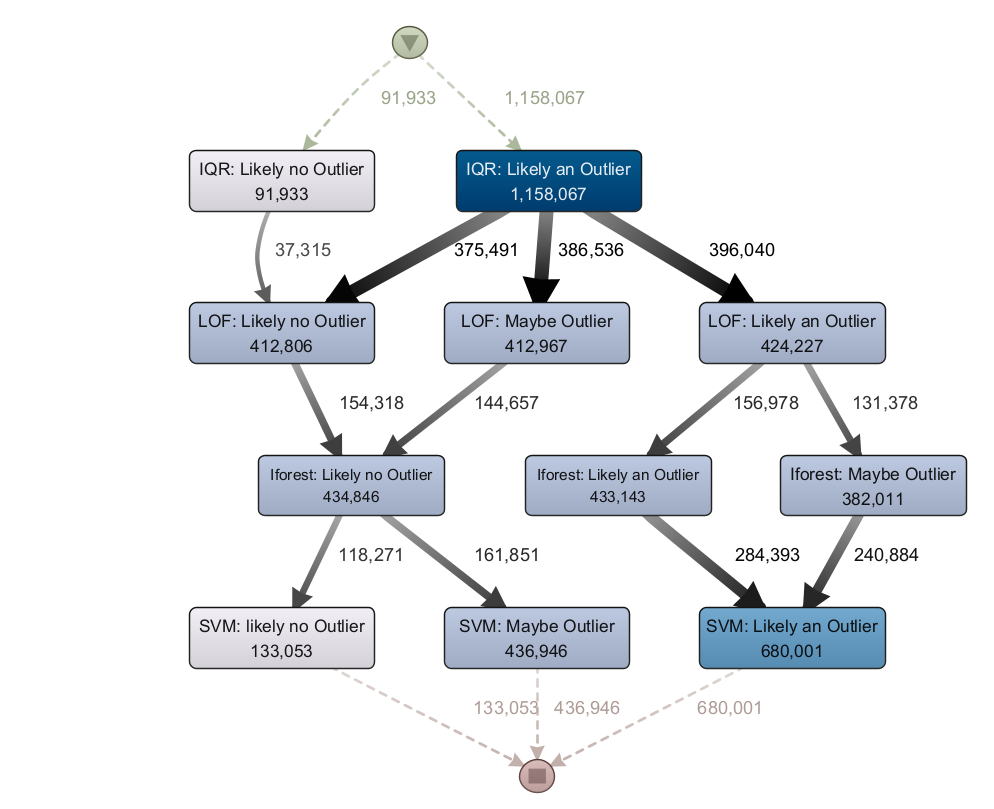
\includegraphics[width=\textwidth]{img/Prozessmodell.png}
	\caption[Prozessmodell]{Prozessmodell}
	\label{fig:Prozessmodell}
\end{figure}